% https://tex.stackexchange.com/a/8935

\documentclass[]{standalone}
\usepackage{standalone}
\usepackage{tikz}
\usetikzlibrary{matrix, positioning, fit,}
\usepackage{lscape}
\usepackage{ifpdf}
\usepackage[\ifpdf\else
hypertex
\fi]{hyperref}

\begin{document}
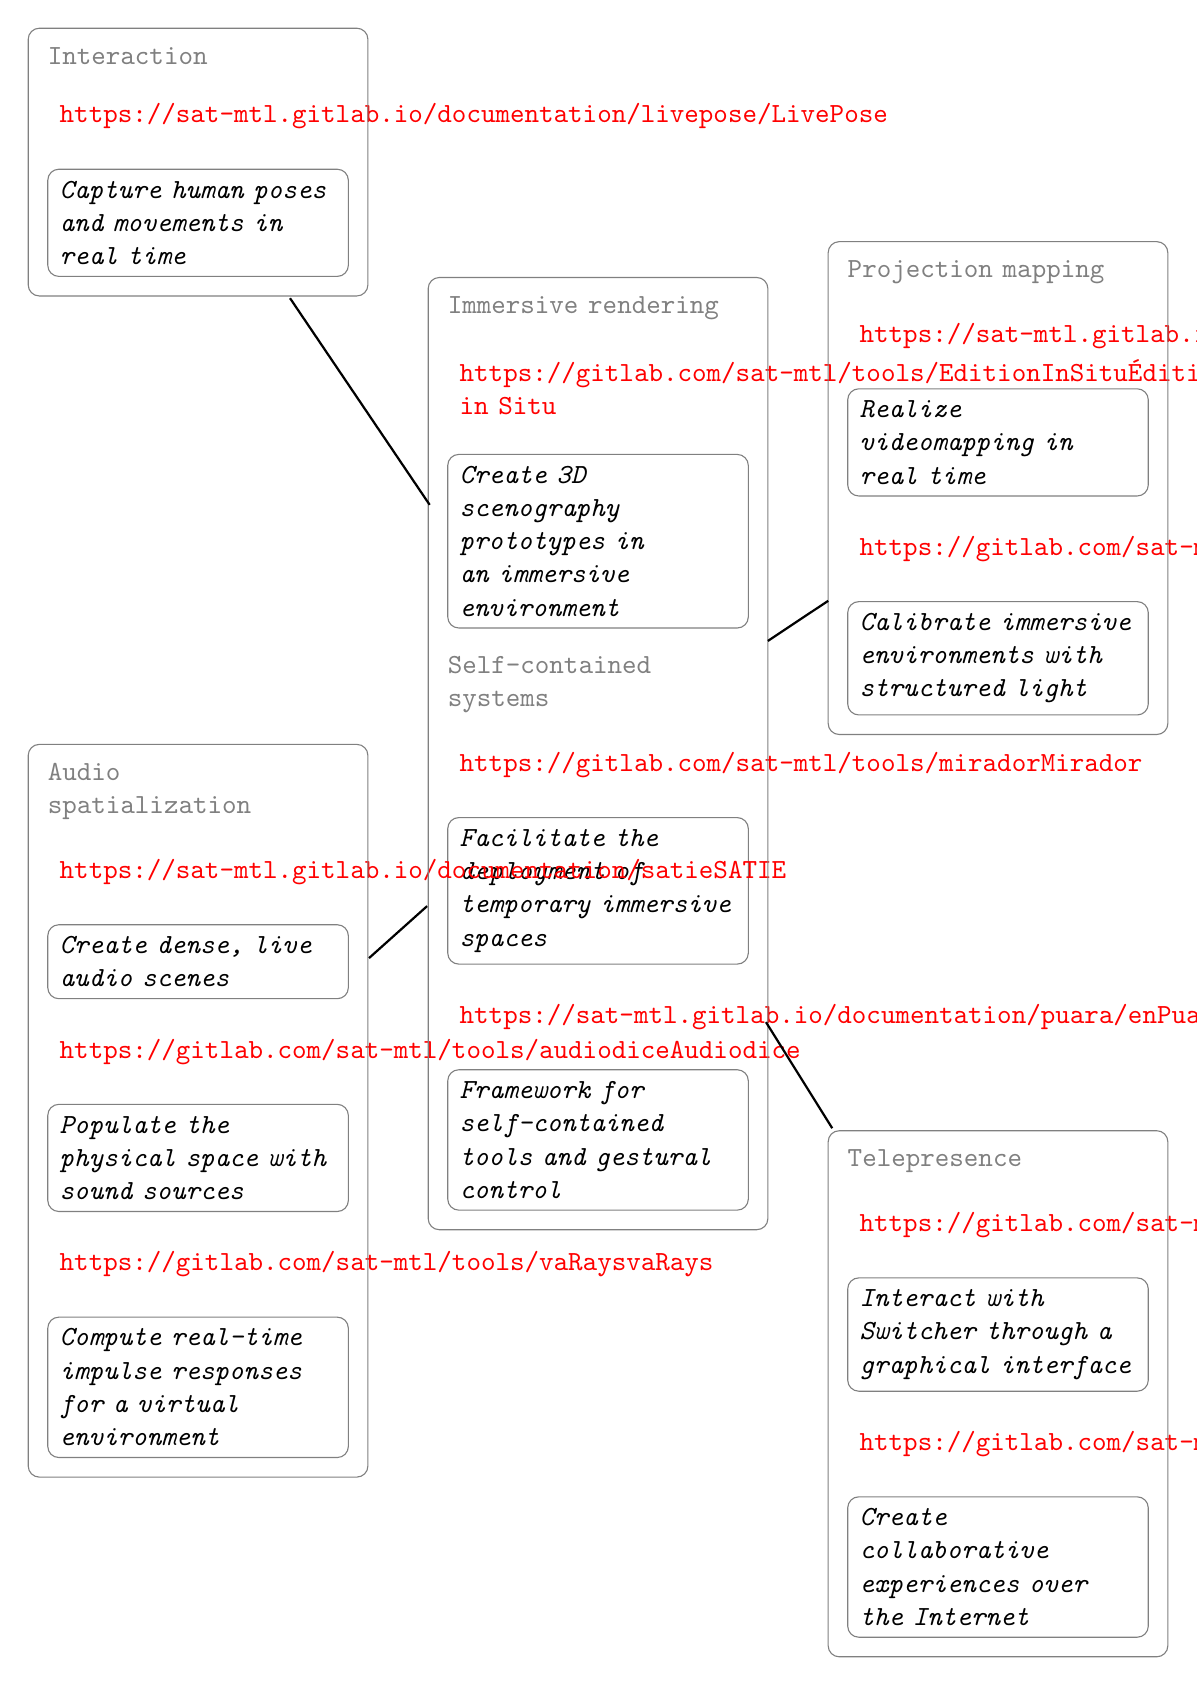
\begin{tikzpicture}[font=\ttfamily,
  mymatrix/.style={matrix of nodes, nodes=typetag, row sep=1em, text width=10em},
  mycontainer/.style={draw=gray, shape=rectangle, rounded corners},
  typetag/.style={draw=gray, shape=rectangle, rounded corners, inner sep=1ex, anchor=west},
  title/.style={draw=none, color=gray, inner sep=0pt},
  subtitle/.style={draw=none, color=red}
  ]
  
  \matrix[mymatrix, matrix anchor=north] (mx1a) {
    |[title]|Immersive rendering \\
    |[subtitle]|\href{https://gitlab.com/sat-mtl/tools/EditionInSitu}{Édition in Situ}\\
    \textit{Create 3D scenography prototypes in an immersive environment} \\
    |[title]|Self-contained systems \\
    |[subtitle]|\href{https://gitlab.com/sat-mtl/tools/mirador}{Mirador}\\
    \textit{Facilitate the deployment of temporary immersive spaces} \\
    |[subtitle]|\href{https://sat-mtl.gitlab.io/documentation/puara/en}{Puara}\\
    \textit{Framework for self-contained tools and gestural control} \\
  };
  
  \matrix[mymatrix, left=of mx1a.north west, anchor=south east] (mx1e) {
    |[title]|Interaction \\
    |[subtitle]|\href{https://sat-mtl.gitlab.io/documentation/livepose/}{LivePose}\\
    \textit{Capture human poses and movements in real time} \\
  };
  
  \matrix[mymatrix, right=of mx1a.base east, anchor=north west] (mx1) {
    |[title]|Telepresence \\
    |[subtitle]|\href{https://gitlab.com/sat-mtl/tools/scenic}{Scenic}\\
    \textit{Interact with Switcher through a graphical interface} \\
    |[subtitle]|\href{https://gitlab.com/sat-mtl/tools/switcher}{Switcher}\\
    \textit{Create collaborative experiences over the Internet} \\
  };
  
  \matrix[mymatrix, left=of mx1a.west, anchor=north east] (mx1d) {
    |[title]|Audio spatialization \\
    |[subtitle]|\href{https://sat-mtl.gitlab.io/documentation/satie}{SATIE}\\
    \textit{Create dense, live audio scenes} \\
    |[subtitle]|\href{https://gitlab.com/sat-mtl/tools/audiodice}{Audiodice}\\
    \textit{Populate the physical space with sound sources} \\
    |[subtitle]|\href{https://gitlab.com/sat-mtl/tools/vaRays}{vaRays}\\
    \textit{Compute real-time impulse responses for a virtual environment} \\
  };
  
  \matrix[mymatrix, right=of mx1a.10, anchor=south west] (mx1b) {
    |[title]|Projection mapping \\
    |[subtitle]|\href{https://sat-mtl.gitlab.io/documentation/splash}{Splash}\\
    \textit{Realize videomapping in real time} \\
    |[subtitle]|\href{https://gitlab.com/sat-mtl/tools/splash/calimiro}{Calimiro}\\
    \textit{Calibrate immersive environments with structured light} \\
  };
  
  \node[mycontainer, fit=(mx1)] {};
  \node[mycontainer, fit=(mx1a)] {};
  \node[mycontainer, fit=(mx1b)] {};
  \node[mycontainer, fit=(mx1d)] {};
  \node[mycontainer, fit=(mx1e)] {};

  \draw[thick, shorten >=5pt, shorten <=5pt] (mx1e) -- (mx1a);
  \draw[thick, shorten >=5pt, shorten <=5pt] (mx1) to (mx1a);
  \draw[thick, shorten >=5pt, shorten <=5pt] (mx1d) to (mx1a);
  \draw[thick, shorten >=4pt, shorten <=4pt] (mx1b) to (mx1a);
       
\end{tikzpicture}
\end{document}

